
%(BEGIN_QUESTION)
% Copyright 2009, Tony R. Kuphaldt, released under the Creative Commons Attribution License (v 1.0)
% This means you may do almost anything with this work of mine, so long as you give me proper credit

Connect a loop-powered differential pressure transmitter (4-20 mA output) to a DC voltage source, a 250 ohm resistor, and a diode as shown, using parts supplied by the instructor.  You will need to bring your multimeter as well as a 4-20 mA loop calibrator for this experiment!  All electrical connections must be made using a terminal strip (no twisted wires, crimp splices, wire nuts, spring clips, or ``alligator'' clips permitted):

$$\includegraphics[width=15.5cm]{i03880x01.eps}$$

\vskip 10pt

When you have your transmitter powered and functioning, answer the following questions:

\begin{itemize}
\item{} Demonstrate how to measure the transmitter's signal using a voltmeter connected in parallel with the 250 ohm resistor.  Leave the voltmeter connected for the duration of the experiment.
\vskip 10pt
\item{} Demonstrate how to use the loop calibrator in the ``Measure'' (or ``Read'') mode to measure the amount of current output by the transmitter.  Compare the loop calibrator's current measurement against the voltmeter's voltage measurement.
\vskip 10pt
\item{} Remove the transmitter from the circuit and replace it with the loop calibrator, then demonstrate how to use the loop calibrator in the ``Simulate'' mode to mimic the operation of the transmitter.  Compare the loop calibrator's current simulation value against the voltmeter's voltage measurement.
\vskip 10pt
\item{} Remove the batteries and the transmitter from the circuit and replace both with the loop calibrator, then demonstrate how to use the loop calibrator in the ``Source'' mode to supply current through the resistor and diode.  Compare the loop calibrator's current source value against the voltmeter's voltage measurement.
\end{itemize}

\underbar{file i03880}
%(END_QUESTION)





%(BEGIN_ANSWER)


%(END_ANSWER)





%(BEGIN_NOTES)

\vskip 20pt \vbox{\hrule \hbox{\strut \vrule{} {\bf Virtual Troubleshooting} \vrule} \hrule}

This question is a good candidate for a ``Virtual Troubleshooting'' exercise.  Presenting the diagram to students, you first imagine in your own mind a particular fault in the system.  Then, you present one or more symptoms of that fault (something noticeable by an operator or other user of the system).  Students then propose various diagnostic tests to perform on this system to identify the nature and location of the fault, as though they were technicians trying to troubleshoot the problem.  Your job is to tell them what the result(s) would be for each of the proposed diagnostic tests, documenting those results where all the students can see.

During and after the exercise, it is good to ask students follow-up questions such as:

\begin{itemize}
\item{} What does the result of the last diagnostic test tell you about the fault?
\item{} Suppose the results of the last diagnostic test were different.  What then would that result tell you about the fault?
\item{} Is the last diagnostic test the best one we could do?
\item{} What would be the ideal order of tests, to diagnose the problem in as few steps as possible?
\end{itemize}


%INDEX% Differential pressure transmitter circuit

%(END_NOTES)


